\documentclass[12pt]{article}

\usepackage{amsmath,amsthm,amsfonts,amssymb,amsxtra}
\usepackage{pgf,tikz}
\usetikzlibrary{arrows,calc}
\renewcommand{\theenumi}{(\alph{enumi})} 
\renewcommand{\labelenumi}{\theenumi}

\pagestyle{empty}
\setlength{\textwidth}{7in}
\setlength{\oddsidemargin}{-0.5in}
\setlength{\topmargin}{-1.0in}
\setlength{\textheight}{9.5in}

\theoremstyle{definition}
\newtheorem{problem}{Problem}

\begin{document}

\noindent{\large\bf MATH 141}\hfill{\large\bf Test\#4.}\hfill{\large\bf
  Fall 2016}\hfill{\large\bf Page 1/4}\hrule

\bigskip
\begin{center}
  \begin{tabular}{|ll|}
    \hline & \cr
    {\bf Name: } & \makebox[12cm]{\hrulefill}\cr & \cr
    {\bf VIP ID:} & \makebox[12cm]{\hrulefill}\cr & \cr
    \hline
  \end{tabular}
\end{center}
\begin{itemize}
\item Write your name and VIP ID in the space provided above.
\item This booklet has four (4) pages, including this one.  
\item You have seventy-five (75) minutes to complete both tests.
\item \textbf{There are four problems in page~2: two are on \emph{related rates}, and two on \emph{optimization} (not necessarily in that order!).  Chose one of each: do the related rates problem on page~3, and the optimization problem on page~4.}
\item The technical part of the optimization problem counts towards 20\% of Test\#3.
\item You must show sufficient work to justify all answers unless
  otherwise stated in the problem.  Correct answers with inconsistent
  work may not be given credit.
\item Credit for each problem is given in parentheses at the right of
  the problem number.
\item No books or notes may be used on this test.  You may use a calculator, if you want.
\end{itemize}
\hrule

\begin{center}
  \begin{tabular}{|c|c|c|}
    \hline
    &&\cr
    {\large\bf Page} & {\large\bf Max.~points} & {\large\bf Your points} \cr
    &&\cr
    \hline
    &&\cr
    {\Large 3} & \Large 50 & \cr
    &&\cr
    \hline
    &&\cr
    {\Large 4} & \Large $50 \lvert 20$ & \cr
    &&\cr
   \hline\hline
    &&\cr
    {\large\bf Total} & \Large $100 \lvert 20$ & \cr
    &&\cr
    \hline
  \end{tabular}
\end{center}
\newpage

%%%%%%%%%%%%%%%%%%%%%%%%%%%%%%%%%%%%% Page 1
\noindent{\large\bf MATH 141}\hfill{\large\bf Test\#4.}\hfill{\large\bf
  Fall 2016}\hfill{\large\bf Page 2/4}\hrule

\bigskip

\begin{problem}[50 pts] 
\large A farmer wants to fence an area of 13.5 million square feet in a rectangular field and then divide it in half with a fence parallel to one of the sides of the rectangle. What should the lengths of the sides of the rectangular field be so as to minimize the cost of the fence?
\end{problem}

\begin{problem}[50 pts] 
\large A street light is mounted at the top of a 15-ft-tall pole.  A man $6~\text{ft}$ tall walks away from the pole with a speed of $7~\text{ft}/\text{s}$ along a straight path.  How fast is the tip of his shadow moving when he is $30~\text{ft}$ from the pole? (leave the answer as a fraction)

\begin{center}
  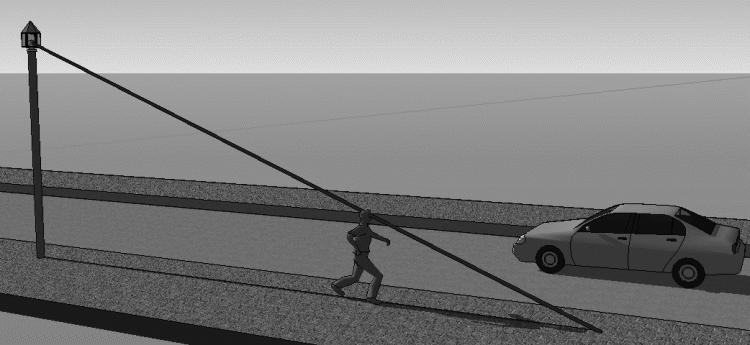
\includegraphics[width=0.5\linewidth]{casey1.png}
\end{center}
\end{problem}

\begin{problem}[50 pts] 
\large At noon, ship $A$ is $70~\text{km}$ west of ship $B$.  Ship $A$ is sailing south at $40~\text{km}/\text{h}$ and ship $B$ is sailing north at $20~\text{km}/\text{h}$.  How fast is the distance between the ships changing at 4:00 PM? (leave the answer as a fraction)
\end{problem}
 
\begin{problem}[50 pts] 
\large A box with square base and open top must have a volume of $4,000~\text{cm}^3$.  Find the dimensions of the box that minimize the amount of material used.

\begin{center}
  \begin{tikzpicture}
  %% Vanishing points for perspective handling
  \coordinate (P1) at (-7cm,1.5cm); % left vanishing point (To pick)
  \coordinate (P2) at (8cm,1.5cm); % right vanishing point (To pick)

  %% (A1) and (A2) defines the 2 central points of the cuboid
  \coordinate (A1) at (0em,0cm); % central top point (To pick)
  \coordinate (A2) at (0em,-2cm); % central bottom point (To pick)

  %% (A3) to (A8) are computed given a unique parameter (or 2) .8
  % You can vary .8 from 0 to 1 to change perspective on left side
  \coordinate (A3) at ($(P1)!.8!(A2)$); % To pick for perspective 
  \coordinate (A4) at ($(P1)!.8!(A1)$);

  % You can vary .8 from 0 to 1 to change perspective on right side
  \coordinate (A7) at ($(P2)!.7!(A2)$);
  \coordinate (A8) at ($(P2)!.7!(A1)$);

  %% Automatically compute the last 2 points with intersections
  \coordinate (A5) at
    (intersection cs: first line={(A8) -- (P1)},
          second line={(A4) -- (P2)});
  \coordinate (A6) at
    (intersection cs: first line={(A7) -- (P1)}, 
          second line={(A3) -- (P2)});

  %%% Depending of what you want to display, you can comment/edit
  %%% the following lines

  %% Possibly draw back faces

  \fill[gray!90] (A2) -- (A3) -- (A6) -- (A7) -- cycle; % face 6
  %\node at (barycentric cs:A2=1,A3=1,A6=1,A7=1) {\tiny f6};
  
  \fill[gray!50] (A3) -- (A4) -- (A5) -- (A6) -- cycle; % face 3
  %\node at (barycentric cs:A3=1,A4=1,A5=1,A6=1) {\tiny f3};
  
  \fill[gray!30] (A5) -- (A6) -- (A7) -- (A8) -- cycle; % face 4
  %\node at (barycentric cs:A5=1,A6=1,A7=1,A8=1) {\tiny f4};
  
  \draw[thick,dashed] (A5) -- (A6);
  \draw[thick,dashed] (A3) -- (A6);
  \draw[thick,dashed] (A7) -- (A6);

  %% Possibly draw front faces

  % \fill[orange] (A1) -- (A8) -- (A7) -- (A2) -- cycle; % face 1
  % \node at (barycentric cs:A1=1,A8=1,A7=1,A2=1) {\tiny f1};
  \fill[gray!50,opacity=0.2] (A1) -- (A2) -- (A3) -- (A4) -- cycle; % f2
  %\node at (barycentric cs:A1=1,A2=1,A3=1,A4=1) {\tiny f2};
  \fill[gray!90,opacity=0.2] (A1) -- (A4) -- (A5) -- (A8) -- cycle; % f5
  %\node at (barycentric cs:A1=1,A4=1,A5=1,A8=1) {\tiny f5};

  %% Possibly draw front lines
  \draw[thick] (A1) -- (A2);
  \draw[thick] (A3) -- (A4);
  \draw[thick] (A7) -- (A8);
  \draw[thick] (A1) -- (A4);
  \draw[thick] (A1) -- (A8);
  \draw[thick] (A2) -- (A3);
  \draw[thick] (A2) -- (A7);
  \draw[thick] (A4) -- (A5);
  \draw[thick] (A8) -- (A5);
  
  % Possibly draw points
  % (it can help you understand the cuboid structure)
  \foreach \i in {1,2,...,8}
  {
    \draw[fill=black] (A\i) circle (0.15em);
  }
  % \draw[fill=black] (P1) circle (0.1em) node[below] {\tiny p1};
  % \draw[fill=black] (P2) circle (0.1em) node[below] {\tiny p2};
\end{tikzpicture}
\end{center}
\end{problem}
\newpage

%%%%%%%%%%%%%%%%%%%%%%%%%%%%%%%%%%%%% Page 2
\noindent{\large\bf MATH 141}\hfill{\large\bf Test\#4.}\hfill{\large\bf
  Fall 2016}\hfill{\large\bf Page 3/4}\hrule

\bigskip
\noindent \textbf{\large Related Rates}
\newpage

%%%%%%%%%%%%%%%%%%%%%%%%%%%%%%%%%%%%% Page 3
\noindent{\large\bf MATH 141}\hfill{\large\bf Test\#4.}\hfill{\large\bf
  Fall 2016}\hfill{\large\bf Page 4/4}\hrule

\bigskip
\noindent \textbf{\large Optimization}

\small{\textbf{Note:} The relevant part related to optimization of this problem will count as 20\% of your exam \#3.}


\end{document}
